\chapter{Adding custom peripherals} \label{ch:AddCustomPeripheral}
\chapterquote{Everyone who drinks this water will be thirsty again, but whoever drinks the water I give them will never thirst.}{Jesus}

\graphicspath{{Chapters/NiosCustomIO/Figures/}}
\lstinputpath{Codes-Verilog/Chapter-Adding-Custom-Peripheral} %path is defined in mypreamble


\section{Introduction}
In previous chapters, only predefined peripherals e.g. JTAG UART and onchip memory etc. are used in the designs. In this chapter, we will learn to add the custom peripherals in the designs. More specifically, clock-tick generator circuit is added in the system, which is described in \href{http://pythondsp.blogspot.com/2016/10/chapter-5-verilog-visual-verifications.html#5.4-Clock-ticks}{`clockTick.v' file of the tutorial `Visual verifications of designs'}. This file is used to reduce the clock rate for the LEDs, so that blinking LED can be seen without adding the dummy loop as well. In the other words, blinking LEDs can be seen for `0000-0000' switch pattern. 

\section{Add custom peripheral}
Follow the below steps to add the custom peripheral in the Nios designs, 

\subsection{Include custom design files (i.e. Verilog/VHDL codes) in the project} 
First, copy the verilog files (in which designs are defined) inside the main project directory,  i.e. `clockTick.v' and `modMCounter.v' files. The codes in these files are shown in Listing \ref{verilog:clockTick2} and \ref{verilog:modMCounter2} respectively. \textbf{Note that, these files can be saved in subdirectory inside the project directory as well; but not outside the project directory as codes may not be detected by the Qsys software.}

\lstinputlisting[
caption    = {Clock-tick generator},
language = Verilog,
label      = {verilog:clockTick2}
]{VerilogCodes/clockTick.v}

\lstinputlisting[
caption    = {Mod-$m$ counter},
language = Verilog,
label      = {verilog:modMCounter2}
]{VerilogCodes/modMCounter.v}


\subsection{Add custom components in Qsys}
Next, we need to create the component in the Qsys design using codes defined in Listing \ref{verilog:clockTick2} and \ref{verilog:modMCounter2}. Follow the below steps for this purpose, 

\begin{enumerate}
	\item First, open the Qsys software and click on File$\rightarrow$New Component.
	\item Next, go to `HDL Files' tab and add the verilog files as shown in Fig. \ref{fig:newClockSource1}. Don't forget to fill the `Top Level Module' column with correct `module name'.
	\begin{figure}[!h]
		\centering
		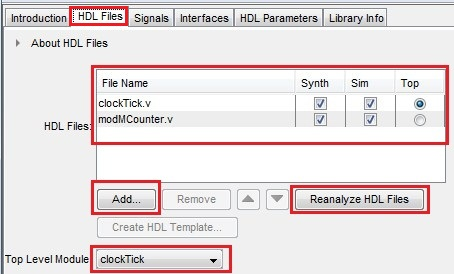
\includegraphics[scale=0.65]{newClockSource1}
		\caption{Add Verilog files in the design}
		\label{fig:newClockSource1}
	\end{figure}
	
	\item Then, go to the `Signals' tab, and select `new Clock Output' and `clk' in columns `Interface' and `Signal type' respectively, for the `clkPulse' as shown in Fig. \ref{fig:newClockSource2} and \ref{fig:newClockSource3}. After these setting, we can use the output of the new component as the clock for other components.
	
	\begin{figure}[!h]
		\centering
		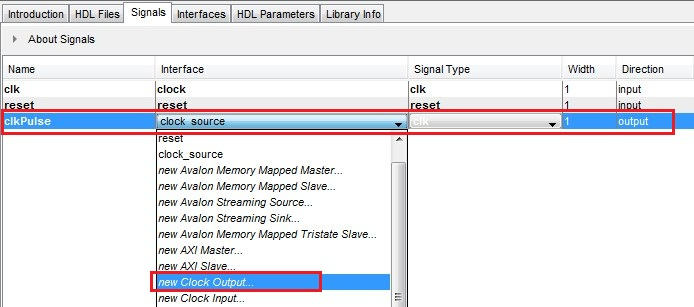
\includegraphics[scale=0.65]{newClockSource2}
		\caption{Change `clkPulse' as `Clock Output'}
		\label{fig:newClockSource2}
	\end{figure}
	\begin{figure}[!h]
		\centering
		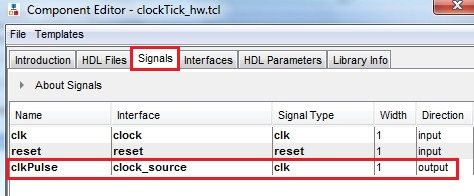
\includegraphics[scale=0.65]{newClockSource3}
		\caption{Final settings for `Signals'}
		\label{fig:newClockSource3}
	\end{figure} 
	
	\item Next, go to the `Interfaces' tab, and remove the unconnected interfaces from the system by clicking on `Remove Interfaces With No Signals' as shown in Fig. \ref{fig:newClockSource4}. This is required because, we change the `interface' type in previous step i.e. `New Clock Output', and Qsys does not remove the `old interface type' automatically.
	\begin{figure}[!h]
		\centering
		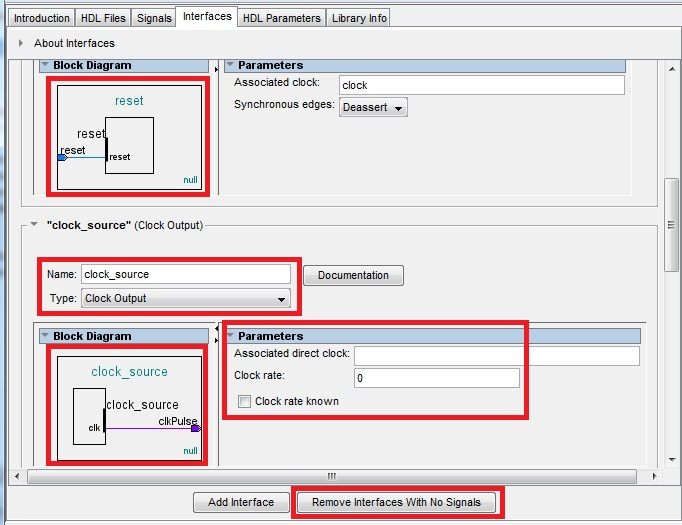
\includegraphics[scale=0.65]{newClockSource4}
		\caption{Remove interfaces with no signals}
		\label{fig:newClockSource4}
	\end{figure} 
	
	\item Note that, two parameters i.e. $M = 5$ and $N = 3$ are defined in Lines 8 and 9 of Listing \ref{verilog:clockTick2}. Default values of these parameters can be changed in the `HDL Parameter' tab as shown in Fig. \ref{fig:newClockSource5}. We did not change the default values in this step, as these values can be modified after adding the component in the system as well.
	\begin{figure}[!h]
		\centering
		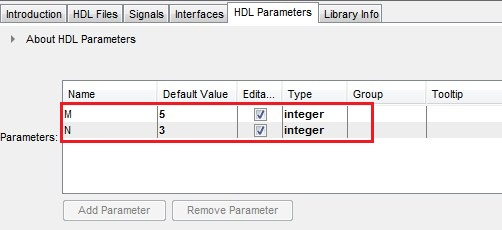
\includegraphics[scale=0.65]{newClockSource5}
		\caption{Modify `parameters'}
		\label{fig:newClockSource5}
	\end{figure} 
	
	\item Finally, add the details for the component as shown in Fig. \ref{fig:newClockSource6} and click on `Finish' button. These details are displayed, while adding the component in the system. Note that, `Display Name' and `Group Name' are filled as `clockTick' and `Meher' respectively, therefore component is displayed as `clockTick' in the `Meher' library as shown in the figure.
	\begin{figure}[!h]
		\centering
		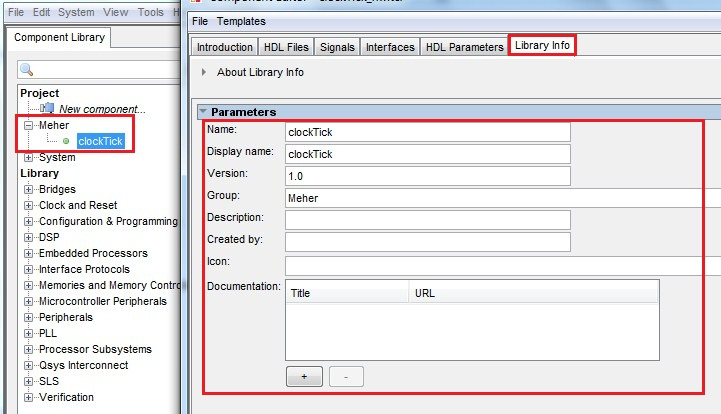
\includegraphics[scale=0.65]{newClockSource6}
		\caption{Add details of component}
		\label{fig:newClockSource6}
	\end{figure}
\end{enumerate}

\subsection{Use custom component in design}
Now, the `clockTick' component can be used in the system which is designed in Chapter \ref{ch:ReadSwitch}. `Double click' on the `clockTick' component and change the default parameter as shown in Fig. \ref{fig:clockTick10ms}. Since value of $M$ is set to `5,00,000', therefore clock is scaled by this factor and resultant clock has frequency 100 Hz (i.e. $50MHz/5,00,000 = 100 Hz)$. In the other words, clock-ticks will be generated at every 10 ms (i.e. $1/100Hz = 0.01 sec)$. 
\begin{figure}[!h]
	\centering
	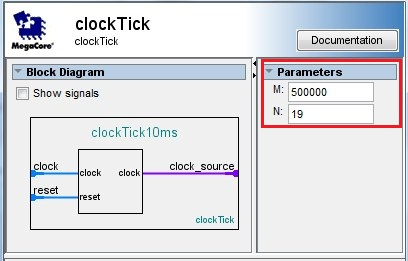
\includegraphics[scale=0.65]{clockTick10ms}
	\caption{Change default parameter for `10ms' clock-tick}
	\label{fig:clockTick10ms}
\end{figure}

Next, rename the component as `clockTick10ms' and add the output-clock of this component as the input-clock for `LEDs' as shown in Fig. \ref{fig:Qsys}. After this, the value of LED port will be read/modified on this new clock of 10 ms. Finally, click on \textbf{`Generate'} button to generate the necessary files for `Quartus' and `Nios' softwares. 
\begin{figure}[!h]
	\centering
	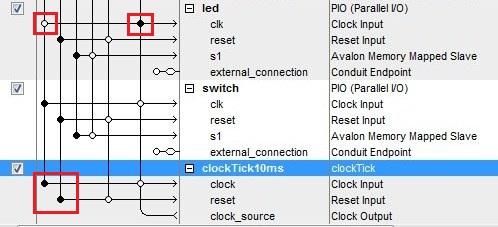
\includegraphics[scale=0.65]{Qsys}
	\caption{Modify LED clock}
	\label{fig:Qsys}
\end{figure}

\begin{noNumBox}
	Note that, this clock can be used for all other components as well except `Nios II processor; as Nios processor requires at least 20 MHz frequency for operation. Further, if the new clock is greater that 20 MHz, then in Fig. \ref{fig:newClockSource4}, `clock rate' must be changed from `0' to new clock rate, otherwise it will generated error for Nios processor as processor requires exact knowledge of the clock frequency.
\end{noNumBox}
\section{Simulate and implement}
Since, no external port is added in the design, therefore no need to change the top level design in Quartus-project. Also, no change is required in `main.c' file in Nios project. The only difference in the design in Chapter \ref{ch:ReadSwitch} and current design is that the LEDs have clock pulses with different time periods. Since, lower frequency clocks are used in this chapter, therefore we can see the blinking LEDs for switch pattern `0000-0000' as well (which was not the case in Chapter \ref{ch:ReadSwitch}, because clock-rate for `0000-0000' pattern was 50 MHz).

Now, Simulate the Nios system and add the waves in the Modelsim as shown in Fig. \ref {fig:AddWave}. Finally, run the simulation for `160 ms' to observe the results which are shown in Fig. \ref{fig:FinalSimulationClockTick}. Note that, in simulation results, the LED-patterns are changing after every 30 ms (not on each clock-tick i.e. 10 ms). This is happening because certain clocks are required for reading and writing operations on LED ports. Lastly, the blinking LEDs can be seen on the FPGA board after loading the `.sof' and `.elf' files on the FGPA chip. 

\begin{figure}[!h]
	\centering
	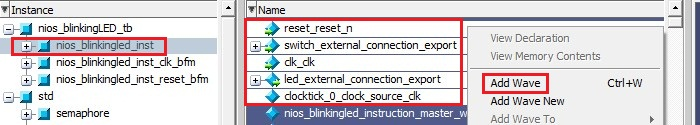
\includegraphics[scale=0.65]{AddWave}
	\caption{Add wave to systems}
	\label{fig:AddWave}
\end{figure}

\begin{figure}[!h]
	\centering
	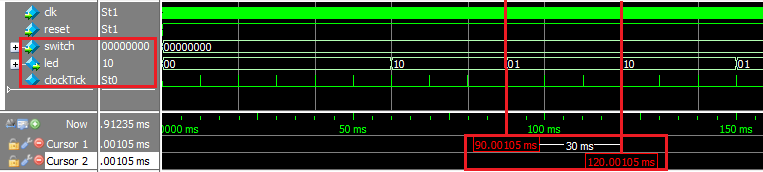
\includegraphics[scale=0.65]{FinalSimulationClockTick}
	\caption{Simulation results}
	\label{fig:FinalSimulationClockTick}
\end{figure}

\section{Conclusion}
In this chapter, we added custom peripheral i.e. `clock-tick generator' in the Qsys software. Further, the default values of the parameters are modified after adding the component in the system. Finally, new clock is used to operate the LEDs and results are verified using simulations.  
